% Setup
\documentclass[11pt]{report}

\usepackage{graphicx, changepage}
\graphicspath{{images/}}

\usepackage{fancyhdr}
\usepackage{etoolbox}

% Layout margins
\usepackage[
  a4paper,
  top     = 2cm,
  bottom  = 3cm,
  left    = 4cm,
  right   = 2cm
]{geometry}

\usepackage[utf8]{inputenc}
\usepackage{helvet}
\usepackage{titlesec}

\renewcommand{\familydefault}{\sfdefault}

% Headings
\titleformat
  {\chapter}
  [hang]
  {\bfseries}
  {\thechapter}
  {12pt}
  {}
\titlespacing
  {\chapter}
  {0pt}
  {10pt}
  {9pt}

\titleformat
  {\section}
  {}
  {\thesection}
  {11pt}
  {}
\titlespacing
  {\section}
  {0pt}
  {0pt}
  {9pt}

\titleformat
  {\subsection}
  {}
  {\thesubsection}
  {11pt}
  {}
\titlespacing
  {\subsection}
  {0pt}
  {0pt}
  {3pt}
  
% Paragraphs
\setlength{\parindent}{0cm}
\setlength{\parskip}{19pt}
\renewcommand{\baselinestretch}{1.3}

% Quote
\patchcmd
  {\quote}
  {\rightmargin}
  {\leftmargin 2.5cm \rightmargin}
  {}{}
\AtBeginEnvironment{quote}{
  \fontsize{10pt}{10pt}\selectfont
}

\newenvironment
  {bullet-list}
  {\begin{itemize}
    [leftmargin=*,
    labelindent=36pt,
    labelsep=1cm]
  }
  {\end{itemize}}
\pagestyle{fancy}

\lhead{}
\rhead{\thepage}
\renewcommand{\headrulewidth}{0pt}

\cfoot{}

\fancypagestyle{plain}{
  \rhead{\thepage}
}

\usepackage{enumitem}
\usepackage{amsmath}

\usepackage{tabularx}

\usepackage[utf8]{inputenc}
\usepackage[T1]{fontenc}
\usepackage[finnish]{babel}

\usepackage{hyperref}

\usepackage[dvipsnames]{xcolor}
\usepackage{listings}
\lstloadlanguages{Ruby}
\lstset{
  basicstyle=\ttfamily\color{black},
  commentstyle = \ttfamily\color{gray},
  keywordstyle=\ttfamily\color{red},
  stringstyle=\color{blue},
  showstringspaces=false
}
\renewcommand{\lstlistingname}{Kuvio}

\definecolor{codegray}{gray}{0.9}
\newcommand{\code}[1]{\colorbox{codegray}{\texttt{#1}}}

\lstdefinelanguage{JavaScript}{
  keywords={break, case, catch, continue, debugger, default, delete, do, else, finally, for, function, if, in, instanceof, new, return, switch, this, throw, try, typeof, var, void, while, with, const},
  morecomment=[l]{//},
  morecomment=[s]{/*}{*/},
  morestring=[b]',
  morestring=[b]",
  morestring=[b]`,
  sensitive=true
}

\usepackage{csquotes}

\begin{document}
  \fancypagestyle{cover}{
   \fancyhf{}
   \rfoot{
     
\includegraphics[width=3cm]{metropolia-logo}   
   }
}

\begin{titlepage}
  \thispagestyle{cover}
  \vspace*{0.3 \paperheight}
  
  {\Large Henrik Raitasola}
  
  {\huge Kehitysympäristön virtualisointi}
  \vspace{2cm}

  \begin{adjustwidth}{-8.2cm}{}
    
\includegraphics[]{line}
  \end{adjustwidth}
  
  Metropolia Ammattikorkeakoulu \\
  Insinööri (AMK) \\
  Tietotekniikka \\
  Insinöörityö \\
  \today
\end{titlepage}
	
  \fancypagestyle{abstract}{
   \rhead{Tiivistelmä}
   \lfoot{
     \begin{adjustwidth}{-4.2cm}{5cm}
       
\includegraphics[]{line-with-metropolia-logo}
     \end{adjustwidth}  
   }
   \setlength{\footskip}{5pt}
}

\fancypagestyle{abstract-english}{
   \rhead{Abstract}
   \lfoot{
     \begin{adjustwidth}{-4.2cm}{5cm}
       
\includegraphics[]{line-with-metropolia-logo}
     \end{adjustwidth}  
   }
   \setlength{\footskip}{5pt}
}

\chapter*{Tiivistelmä}
\thispagestyle{abstract}

\begin{tabular}{|l|l|l|}
  \hline
  Tekijä(t) & Henrik Raitasola \\
  Otsikko & Kehitysympäristön virtualisointi \\
  ~ & ~ \\
  Sivumäärä & \pageref{LastPage} sivua \\
  Aika & \today \\
  \hline
  Tutkinto & Insinööri (AMK) \\
  \hline
  Koulutusohjelma & Tietotekniikka \\
  \hline
  Suuntautumisvaihtoehto & Ohjelmistotekniikka \\
  \hline
  Ohjaaja(t) & Lehtori Ilpo Kuivanen \\
  \hline
  \multicolumn{2}{| p{\textwidth} |}{Tämän insinöörityön aiheena oli ratkaista yleisimpiä kehittäjien ongelmia, jotka liittyvät kehitysympäristöön. Usein ongelmat johtuvat kehittäjien tietokoneiden erilaisuuksista, kuten käyttöjärjestelmästä ja siihen asennettujen projektikohtaisten riippuvuuksien eriävistä versioista. Yleisin lausahdus on \enquote{Toimii minun koneellani}, kun mystisestä syystä samalla tavalla asennettu kehitysympäristö toimii toisella kehittäjällä ja toisella ei. Ongelmia halutaan ratkaista virtualisoimalla kehitysympäristö. \newline

Kehitysympäristö virtualisoitiin ensin Vagrantin avulla. Vagrant loi virtuaalikoneita, johon asennettiin shell-skriptin avulla halutut projektin riippuvuudet. Sen jälkeen tehtiin monimutkaisempi esimerkki Ansiblen avulla, joka toimii hyvin yhteistyössä Vagrantin kanssa. Ansiblella tehtiin playbookeja, joilla pystyy selkeämmin jakamaan riippuvuuksien asennuksen omiin rooleihin. Tämä on selkeämpi lähestymistapa pelkkiin shell-skripteihin verrattuna. \newline

Lopputuloksena esiteltiin muutamia eri kehitysympäristöjen asennuksia. Nämä virtuaaliset kehitysympäristöt minimoivat ongelmia, jotka esiintyvät yleisimmin, kun kehittäjillä ei ole yhteistä virtuaalikehitysympäristöä. 

} \\
  \hline
  Avainsanat & Virtualisointi, Vagrant, Ansible \\
  \hline
\end{tabular}

\chapter*{Abstract}
\thispagestyle{abstract-english}

\begin{tabular}{|l|l|l|}
  \hline
  Author(s) & Henrik Raitasola \\
  Title & Making development environment virtual \\
  ~ & ~ \\
  Number of pages & \pageref{LastPage} pages \\
  Date & \today \\
  \hline
  Degree & Bachelor of  Engineering \\
  \hline
  Degree Programme & Information Technology \\
  \hline
  Specialisation & Software engineering \\
  \hline
  Instructor(s) & Ilpo Kuivanen, Lecturer \\
  \hline
  \multicolumn{2}{| p{\textwidth} |}{The purpose of this thesis was to solve most common development environment problems developers have. Most of the time the problems are caused by the variation of developer's computers such as operating system. Some of the problems are caused by specific project dependencies. The most common comment is \enquote{It works on my machine!} when for mystical reason the same way installed development environment works on other developer's computer and on other's doesn't. These problems are going to be solved by virtualization of development environment.
\newline

Development environment was first virtualizated with Vagrant. Vagrant created virtual machines in which project dependencies were installed by shell-script. Next more complicated example was made with Ansible which worked well with Vagrant. Playbooks were created with Ansible. Playbooks help separating installation of dependencies to own roles. This approach is more clear compared to just shell-scripts.
\newline

As a result couple different installations of development environments were introduced. Virtual development environments minimize problems that are usually caused when developers don't have common virtual environment available.

} \\
  \hline
  Keywords & virtual, Vagrant, Ansible \\
  \hline
\end{tabular}

  \fancypagestyle{table-of-contents}{
   \fancyhf{}
   \lfoot{
     \begin{adjustwidth}{-4.2cm}{5cm}
       
\includegraphics[]{line-with-metropolia-logo}
     \end{adjustwidth}  
   }
   \setlength{\footskip}{5pt}
}

{
  \tableofcontents
  \thispagestyle{table-of-contents}
  \cleardoublepage
}
  
  \setcounter{page}{1}
  
  \chapter{Johdanto}

Kuvitellaan, että aloitteleva kehittäjä Klaus tekee ensimmäistä tietokannallista nettisivuprojektia PHP:lla ilman ulkoisia kirjastoja. PHP-koodi ajetaan paikallisella Apache-palvelimella ja kaikki sujuu ongelmitta. Projektiin liittyy myöhemmin toinen kehittäjä Pekka. Uusi kehittäjä pääsee helposti mukaan, sillä kehitysympäristö on vielä yksinkertainen. Projektista yksinkertaisen tekee yleisesti käytetty käytetty LAMP-kehitysympäristö ja se, että ulkoisia kirjastoja ei toistaiseksi ole.

Myöhemmin Klaus aloittaa uuden Node-projektin ja kutsuu Pekan jälleen mukaan tiimiin. Vanhasta kokemuksesta kehitysympäristön pitäisi toimia yhtä hyvin kuin edellisessä PHP-projektissakin. Klaus antaa Pekalle seuraavat ohjeet: asenna Node, kloonaa projekti ja asenna riippuvuudet. Tämän tehtyää Pekka huomaa, että riippuvuudet eivät asennu. Eikä ongelman ratkaisemiseksi auta kryptinen virheilmoituskaan. Molemmat kehittäjät selvittävät vikaa muutaman päivän ajan ja lopulta selvisi, että Pekalla oli uudempi versio Nodesta, jota yksi riippuvuuksista ei tukenut.

Tämä inssityö auttaa ratkaisemaan samankaltaisia ongelmia tekemällä  kehitysympäristön asentamisesta automaattisen. Käytännössä tämä tarkoittaa, että kehitysympäristö on virtuaalinen, joten omalle fyysiselle tietokoneelle asenneta projektikohtaisia riippuvuuksia. Insinöörityössä kerrotaan mitä ovat Vagrant ja Ansible, ja miten niillä voidaan ratkaista yleisimpiä kehitysympäristön ongelmia.

Insinöörityön tavoitteena on luoda virtuaalisiakehitysympäristöjä, joita voidaan jakaa projektin jäsenien kesken ja joita helppo pystyttää ilman oman koneen saastuttamista.

	
  \chapter{Kehitysympäristö}

\section{Ongelma}
Yleisin ongelma usean kehittäjän tiimissä on kehitysympäristön erilaisuus. Tämä ilmenee parhaiten kun kehittäjät käyttävät työkoneellaan eri käyttöjärjestelmiä kuten Linuxia, OS X:ää ja Windowsia. Usein projekteissa on pitkät asennusohjeet, jossa kerrotaan tarkasti mitkä riippuvuudet pitää asentaa sekä niiden tarkat versionumerot. Usein riippuvuuksien asennus on erilaista riippuen käyttöjärjestelmästä. Ei ole epätavallista, että ympäristön pystytykseen voi mennä muutama työpäivä. Oman kokemukseni mukaan pystytysprosessiin menee paljon henkilötyötunteja, sillä lähes aina tarvitaan apua projektissa aikaisemmin olleelta henkilöltä.

\section{Ratkaisu}
Jotta kaikille kehittäjille saadaan täysin samanlaiset kehitysympäristöt niin yksi ratkaisu on virtuaalikoneet. VirtualBox tai WMware ovat esimerkkejä virtuaalikoneohjelmista. Virtuaalikoneet ovat täysiverisiä käyttöjärjestelmiä isäntäkoneen eli käyttäjän koneen sisällä. Usein kehityskäyttöjärjestelmäksi valitaan jokin Linux paketti esimerkiksi Ubuntu. Näin kaikille kehittäjille saadaan sama käyttöjärjestelmä, jossa kehitys tapahtuu. Tämä vähentää riippuvuuksien asentamisessa tapahtuvaa virheiden määrää.

Pelkkä käyttöjärjestelmän yhdenmukaistaminen ei riitä sillä riippuvuuksien asentamisessa yleensä ongelmat ilmenevät. Pelkkä VirtualBox ei riitä sillä kaikki siihen halutut ohjelmat pitää asentaa käsin tai tehdä iso kokoinen levykuva, josta asennettaisiin ympäristö.

\section{Vagrant}
Vagrantin avulla voidaan luoda virtuaalikoneita helposti komentoriviltä. Vagrant on yksinkertainen ohjelma, joka vain käskyttää VirtualBoxia. Tästä syystä VirtualBox täytyy olla asennettuna, jotta Vagrant toimii.

Vagranttia kannattaa ajatella vertauskuvan kautta. Kuvitellaan, että Erik haluaa perustaa Subway-ravintolan. Koska Subway on pikaruokaravintolaketju sillä on tarkasti määritelty mitä aineksia ruoka-annoksissa saa käyttää, minkälaiset työvaatteet pitää olla ja miten asiakaspalvelu pitäisi toimia tms. Erik saa itse valita tilan johon perustaa ravintolan. Tilan valitsemisen jälkeen hänen täytyy sisustaa ravintola Subwayn määrittämällä tavalla. Seuraavaksi täytyy hankkia uuni, jääkaappi, mikro ja muut ruuan tekemiseen tarkoitetut välineet. Tässä vaiheessa saattaa tulla tilanne, jossa kaikki hankitut laitteet eivät välttämättä sovi valittuun liiketilaan. Esimerkiksi Erikin valitsemalle jääkaappille ei löydy sopivaa paikkaa liiketilasta. Paljon yhteensopivuus ongelmia voi syntyä ennen kuin uusi Subway-ravintola voidaan avata. Tämä on luonnollista, koska Subwayn johto ei voi tietää miten kaikki laitteet menevät mihin tahansa liiketilaan.

Kun Subwayn liikejohto huomasi, että uusilla ravintoloiden perustajilla on usein ongelmia ravintolan pystyttämisessä ja sen saamiseksi ohjeiden mukaiseen kuntoon he päättivät helpottaa asiaa. He kehittivät uusien ravintoloiden perustajille paketin, josta täytyy vain painaa nappia eikä ravintoloitsijan tarvitse tehdä muuta. Erik kokeili uutta asennuspakettia ja huomasi, että paketista tuli ulos robotti, joka lähti heti rakentamaan liiketilaa ravintolalle. Robotti rakentaa aina samanlaisen tyhjän liiketilan johdon määrittelemällä tavalla. Kun liiketila on valmis robotti aloittaa jääkaappien, uunien ja muiden laitteiden asentamisen, jotka ovat välttämättömiä Subway-ravintolan pitäjälle. Kun laitteet ovat asennettu liiketila viimeistellään sisustuksella. Robotti tiesi miten asennukset ja sisustaminen pitää tehdä, koska sille on määritelty ohje, jota se lukee. Kun robotti on tehnyt kaiken se antaa liiketilan avaimet Erikille, jonka ei tarvitse muuta kuin laittaa uunit päälle niin hän voi aloittaa myymisen.

\subsection{Vagrantin toiminta}
Vagrant luo isäntäkoneen sisälle virtuaalikoneen kuten kuvassa \ref{fig:how-vagrant-works}.Virtuaalikone sisältää kaikkille kehittäjille yhteinen käyttöjärjestelmän. Lisäksi Vagrantille annetaan "resepti", jonka mukaan se asentaa kaikki projektin riippuvuudet. Koodin kääntäminen, komentojen ajaminen, mahdollisen tietokannan käyttäminen tms. asiat tehdään virtuaalikoneella. Näin isäntäkone pysyy puhtaana turhista ohjelmista, eikä synny aikaisemmin mainittuja ongelmia. Isäntäkoneessa tapahtuu koodin kirjoittaminen, tiedostojen luonti ja versiohallinan käyttäminen.

\begin{figure}[h]
  \includegraphics[width=\textwidth]{how-vagrant-works}
  \caption{Vagrantin toiminta isäntäkoneen sisällä}
  \label{fig:how-vagrant-works}
\end{figure}

\subsection{Vagrantin käyttäminen}
Ennen Vagrantin käytön aloittamista täytyy VirtualBox ja Vagrant olla asennettuna. Avaamalla terminaalin voit nyt käyttää vagrant-komentoja terminaalissa. Jos komento \code{vagrant -v} palauttaa Vagrantin nykyisen version niin asennus on mennyt oikein. Tästä eteenpäin työskennellään koko ajan terminaalissa.

Siirry projektikansioon ja aja \code{vagrant init}. Vagrant luo kansioon Vagrantfile-nimisen tiedoston. Vagrantfile on käytännössä Ruby-ohjelmointi kieltä, jota Vagrant osaa lukea kun se ajetaan. Vagrantfilessä voi siis käyttää kaikkia Ruby-kielen toimintoja. Kuviosta \ref{listing:InitialVagrantfile} näkyy tiedoston sisältö ilman kommentteja.

\begin{lstlisting}[
  label=listing:InitialVagrantfile,
  language=Ruby,
  caption=Alustava Vagrantfile,
  float=h
]
Vagrant.configure(2) do |config|
  config.vm.box = "ubuntu/trusty64"
end
\end{lstlisting}

Kaikki virtuaalikoneen asetukset tulevat config-osion sisälle. Tällä hetkellä koneelle määritellään vain boxi: "ubuntu/trusty64". Mahdollisia boxeja voi etsiä osoitteesta: \url{https://atlas.hashicorp.com/boxes/search}. Boxit ovat käytännössä käyttöjärjestelmä eli pohja virtuaalikoneelle. Tässä tapauksessa boxina on Ubuntu, joka perustuu Debian Linux-jakeluun \cite{link:ubuntu}. Boxi on ravintolavertauskuvassa ravintolan liiketila. Boxi on pakko olla, mutta itsessään sillä ei tee paljon mitään. Boxi täytyy "sisustaa" eli asentaa projektiin liittyvät ohjelmat ja riippuvuudet.

Yksinkertaisin keino asentaa ohjelmia virtuaalikoneelle on shell-skriptien avulla. Jos projektiin tarvitsee asentaa vain muutama ohjelma voidaan ne asentaa laittamalla asennus-skripti suoraan Vagrantfileen. 

\begin{lstlisting}[
  label=listing:vagrant-shell-inline,
  language=Ruby,
  caption=Vagrantin yksinkertainen shell-skripti,
  float=h
]
config.vm.provision "shell",
  inline: "apt-get update; apt-get install -y apache2"
\end{lstlisting}

Kuviossa \ref{listing:vagrant-shell-inline} Vagrantfilen sisään on lisätty provisiointi shell-skripti, joka on tyyppiä inline. Tällä tarkoitetaan, että koko skripti annetaan suoraan stringinä. Tässä esimerkissä \code{apt-get update} päivittää virtuaalikoneen lokaalitpaketti linkit. \code{apt-get install -y apache2} tarkoittaa että asennetaan Apache-palvelinohjelma, jota monet käyttävät esimerkiksi PHP-projekteissa. Lippu -y pitää lisätä, koska apt varmistaan usein käyttäjältä, että haluaako hän varmasti asentaa kyseisen paketin. Lippu varmistaa sen, että kaikki pakettiin liittyviin kysymyksiin vastataan kyllä.

Skripti voidaan myös jakaa monelle riville Rubyn HEREDOC:n avulla kuvion \ref{listing:vagrant-shell-heredoc} osoittamalla tavalla. HEREDOC \cite{link:ruby-heredoc} mahdollistaa stringin kirjoittamisen monelle riville, mikä helpottaa luettavuutta kun asennetaan paljon ohjelmia.

\begin{lstlisting}[
  label=listing:vagrant-shell-heredoc,
  language=Ruby,
  caption=Vagrantin shell-skripti HEREDOC:lla,
  float=h
]
config.vm.provision "shell", inline: <<-SHELL
  apt-get update
  apt-get install -y apache2
SHELL
\end{lstlisting}

Käytännössä kuitenkin shell-skripti kannattaa laittaa erilliseen tiedostoon kuten kuviossa \ref{listing:vagrant-shell-path}. Jos Vagrantfile ja shell-skripti ovat samassa kansiossa niin riittää kun laittaa vain skriptin nimen.

Ulkoiseen skriptii täytyy laittaa alkuun kommentti, jossa kerrotaan, että kyseessä on shell-skripti. Ulkoisen skriptiin on helppo määritellä paljon eri ohjelmien asennuksia ja konfigurointeja.

\begin{lstlisting}[
  label=listing:vagrant-shell-path,
  language=Ruby,
  caption=Provisiointi-skripti voi olla myös erillisessä tiedostossa,
  float=h
]
config.vm.provision "shell", path: "install-environment.sh"
\end{lstlisting}

\begin{lstlisting}[
  label=listing:vagrant-external-shell-script,
  language=bash,
  caption=Ulkoinen shell-skripti,
  float=h
]
#!/bin/bash
apt-get update
apt-get install -y apache2
\end{lstlisting}

Koska projektin koodaaminen tehdään host-koneella niin haluamme saada yhteyden esimerkiksi Apache-palvelimeen suoraan host-koneelta. Siksi seuraavaksi pitää avata virtuaalikoneen portteja host-koneelle. Apache vastaa oletuksena osoitteesta \url{http://localhost:80}, joten haluamme avata portin 80 isäntäkoneelle. Vagrantfileen voidaan määrittää mikä virtuaalikoneen portti halutaan ohjata mihin isäntäkoneen porttiin. Kuviossa \ref{listing:vagrant-port-mapping} virtuaalikoneen portti 80 ohjataan isäntäkoneen porttiin 8080.

\begin{lstlisting}[
  label=listing:vagrant-port-mapping,
  language=Ruby,
  caption=Virtuaalikoneen portti 80 ohjataan isäntäkoneen porttiin 8080,
  float=h
]
config.vm.network "forwarded_port", guest: 80, host: 8080
\end{lstlisting}

Nyt kun isäntäkoneella mennään selaimella osoitteeseen \url{http://localhost:8080} niin pitäisi tulla näkyviin Apachen oletussivu jos Apache on asennettu joillakin edellä mainituilla tavoilla virtuaalikoneeseen. Kuvassa \ref{fig:apache-default-page} näkyy Apachen oletussivu kun virtuaalikoneen portit on ohjattu oikein.

\begin{figure}[h]
  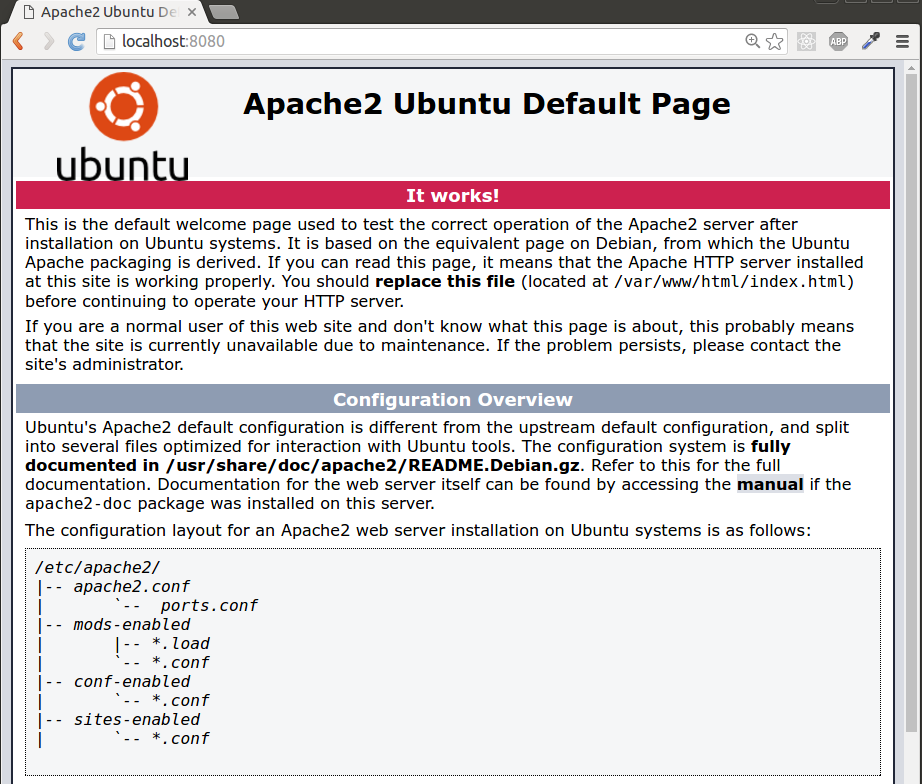
\includegraphics[width=\textwidth]{apache-default-page}
  \caption{Isäntäkone näkee Apachen oletussivun kun oikeat portit ovat auki}
  \label{fig:apache-default-page}
\end{figure}

Nyt kun Apache on asennettu oikein voidaan viedä virtuaalikoneelle projektin tiedostostot. Oletetaan, että projektissa on yksinkertaisuuden vuoksi vain index.html-tiedosto. Kuviossa \ref{listing:vagrant-synced-folder} näytetään miten haluttu kansio saadaan synkronoitua virtuaalikoneeseen.

Ensimmäinen parametri kertoo mikä isäntäkoneen kansio halutaan synkronoida. Polun voi antaa relatiivisena tai absoluuttisena. Tässä tapauksessa parametri on relatiivisesti nykyinen kansio. Toinen parametri kertoo minne kansio halutaan synkronoitua virtuaalikoneessa. Isäntäkoneen kansio halutaan synkronoida kansioon /var/www/html, koska sieltä Apache lukee oletuksena tiedostoja. Nyt kun lisätään projektin juureen isäntäkoneella tiedosto index.html, jonka sisältönä on \code{Hello from project file} saadaan kuvan \ref{fig:index-file-response} mukainen vastaus Apachelta.

\begin{figure}[h]
  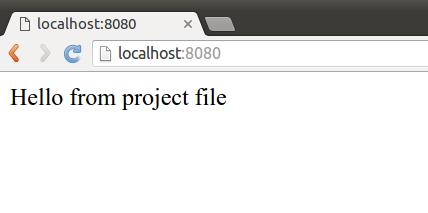
\includegraphics[width=\textwidth]{index-file-response}
  \caption{Apache vastaa index.html tiedoston sisällön}
  \label{fig:index-file-response}
\end{figure}

Vagrant synkronoi tiedostot valittujen kansioiden välillä molempiin suuntiin. Kun tiedosto lisätään isäntäkoneella niin sama tiedosto ilmestyy virtuaalikoneelle. Samoin jos virtuaalikoneelle lisätään tiedosto synkronoituun kansioon niin tämä tiedosto tulee isäntäkoneelle. Työskennellessä on kuitenkin tarkoitus toimia lisäämällä tiedostoja aina isäntäkoneelle.


Jos isäntä- ja virtuaalikoneella on kaksi saman nimistä tiedostoa niin isäntäkoneella oleva tiedosto ylikirjoittaa virtuaalikoneen tiedoston. Esimerkiksi kansiossa /var/www/html on Apachen oletus index.html-tiedosto, mutta projektin index.html ylikirjoittaa sen.

Kuvassa \ref{fig:how-vagrant-works} on visualisoitu kaksisuuntainen kansion synkronointi.

\begin{lstlisting}[
  label=listing:vagrant-synced-folder,
  language=Ruby,
  caption=Isäntäkoneen kansio synkronoidaan virtuaalikoneen kansioon,
  float=h
]
config.vm.synced_folder ".", "/var/www/html"
\end{lstlisting}

Vagrantin hyödyt
\begin{bullet-list}
  \item Ei tarvitse omalle (hosti)koneelle asentaa mitään.
  \item Projektin ympäristön asennustiedot ovat version hallinnassa Vagrantfilessä ja shell-skripteissä.
  \item Ympäristön saa pystyyn vain komentamalla \code{vagrant up}.
  \item Kaikilla kehittäjillä sama ympäristö.
\end{bullet-list}

Vagrantin haitat
\begin{bullet-list}
  \item Virtuaalikoneet vievät välillä enemmän keskusmuistia kuin lokaalisti ajaessa.
  \item Yleensä tarvitsee tehdä lisäsäätöä esimerkiksi ku tarkkaillaan tiedoston muutoksia.
\end{bullet-list}

\subsection{Alaluvun alaotsikko}

Otsikon jälkeen tulee tekstiä tai uusi alaotsikko.

\begin{table}[h]
  \caption{Metropolian opiskelijoiden lukuvuonna 2009–2010 suorittamat virtuaaliopinnot.}
  \begin{tabular}{| l | l | l |}
  \hline
  \bfseries Koulutusala & \bfseries Suoritusten määrä, op \\
  \hline
  Kulttuuriala & 131 \\
  \hline
  Tekniikan ja liikenteen ala & 552 \\
  \hline
  Sosiaali- ja terveysala & 175 \\
  \hline
  Liiketaloudena ala & 52 \\
  \hline
  Ei sidottu koulutusalaan & 18 \\
  \hline
  \bfseries Metropolia yhteensä & \bfseries 928 \\
  \hline
  \end{tabular}
  \label{tab:virtual studies}
\end{table}

Kuvan tai taulukon jälkeen tulee tekstiä ennen uutta kuvaa tai taulukkoa tai seuraavaa otsikkoa.

\subsection{Alaluvun alaotsikko}

Alaluvun alaotsikon jälkeen tulee tekstiä.

Sitaatti toteutetaan Lainaus-tyylillä. Sitaatin johtolauseen sisältävässä kappaleessa (välittömästi sitaattia edeltävässä kappaleessa) käytetään tyyliä ”Leipäteksti ennen lainausta”, jotta sitaatin ja johtolauseen väliin jää lyhyempi kappaleväli.

\begin{quote}
Usean rivin pituinen suora lainaus kirjoitetaan kirjainkoolla 10. Tekstissä käytetään riviväliä 1, ja teksti sisennetään. Suorassa lainauksessa käytetään mallipohjan lainaustyyliä. Lainaukseen merkitään lähdeviite.
\end{quote}
  
  \chapter{Ansible}

Ansible on tarkoitettu palvelinten konfiguraation hallinnoimiseen, palveluiden hallinnointiin ja esimerkiksi web-palveluiden käyttöönottoon ja asentamiseen. Ansiblella voidaan esimerkiksi asentaa kehitys- että tuotantoympäristöön tarvittavat riippuvuudet helposti ja paremmin kuin esimerkiksi shell-skripteillä. Nykyään on myös hyvä tapa tehdä kehitys- että tuotantonympäristöstä mahdollisimman samanlaisia, jotta ympäristöjen erilaisuuksista ei tule ongelmia. Ansiblessa pystyy helposti uudelleen käyttämään siihen määriteltyjä asennustehtäviä parametrisoimalla niitä. Esimerkiksi tietokantayhteys voi hieman poiketa tuotantoympäristössä. Kaikki nämä ja paljon muuta hoituu helposti Ansiblella.

Mietitään jälleen vertauskuvaa Subway-ravintolan perustamisesta. Kun laatikosta tullut robotti on rakentanut ravintolan liiketilan se aloittaa laitteiden asentamisen ja sisustamisen. Jos Erik haluaa myöhemmin esimerkiksi sisustaa ravintolan uudestaan ohjeiden mukaan ollakseen varma, että ravintolan on Subwayn johdon määritelmän mukainen, hänen täytyy kutsua robottia tekemään sisustus uudestaan. Tämä toiminpide täytyy tehdä viimeistään silloin kun Subwayn johto on muuttanut rakennusohjeita.

Vanha robotti tekisi tällöin sekä laitteiden asennuksen, että sisustuksen uudestaan, mutta se saattaa rikkoa paikkoja, koska se esimerkiksi sisustaisi kaiken uudestaan vaikka osa sisustuksesta olisikin jo paikoillaan. Tästä voi luonnollisesti koitua ongelmia ja pahimmassa tapauksessa robotin täytyy tuhota koko ravintola ja aloittaa alusta rakentaminen, laitteiden asennus ja sisustaminen. Toisaalta tämä ei haittaa, koska alusta asti rakennettu ravintola toimii aina. Ainostaan aikaa menee tällöin hukkaan.

Uusi robotti on fiksumpi kuin edellinen. Kun Erik haluaa varmistaa, että ravintola on vanhojen ohjeiden mukainen tai varmistaakseen, että uusimmat muutokset ovat tehty ravintolaan täytyy hänen jälleen kutsua robottia asentamaan ravintola. Ennen kuin uusi robotti alkaa asentaa mitään se tutkii ravintolaa ja kerää siitä tietoa. Kun tiedot on kerätty se aloittaa asentamisen. Esimerkiksi jääkaapin asennuken kohdalla robotti ensin tutkii onko jääkaappi jo asennettu ja jos se on niin se siirtyy seuraavaan asennukseen. Asennuksen päätteeksi robotti ilmoittaa Erikille kuinka monta asiaa asennuslistalta oli jo tehty ja kuinka monta asiaa muutettiin. Esimerkiksi: "10 kohdetta oli jo asennettu ja jääkaapin tilalle asennettiin jääkaappipakastin yhdistelmä".

\section{Ansiblen toiminta}

Ansiblen kaltaisia ohjelmia on muutamia, mutta Ansiblen suosio perustuu sen yksinkertaisuuteen ja keveyteen. Käyttääksesi Ansiblea tarvitset vain Pythonin, SSH-yhteyden kohdekoneeseen ja käyttäjän, joka voi suorittaa skriptejä kohdekoneella \cite{link:what-is-ansible}. Jotta Ansiblen käyttäminen olisi erittäin sujuvaa kannattaa kohdekoneelle lisätä SSH-avain, koska tällöin ei tarvita käyttäjätunnus salasana yhdistelmää kun otetaan yhteyttä kohdekoneeseen.

Jotta Ansible pääsee suorittamaan sille annettuja tehtäviä kohdekoneeseen, täytyy sen ensin ottaa SSH-yhteys kohdekoneeseen. Tämä ei vaadi client-koneelta yleisesti mitään lisäasetuksia. Kun yhteys on saatu kohdekoneeseen kerää Ansible tietoja siitä esimerkiksi käyttäjärjestelmän, mitä paketteja on jo asennettu yms. Sen jälkeen Ansible lähtee ajamaan sille määriteltyjä tehtäviä kohdekoneelle. Tehtävät määritellään playbookkeina, jotka sijaitsevat client-koneella \ref{fig:how-ansible-works}

\begin{figure}[h]
  \includegraphics[width=\textwidth]{how-ansible-works}
  \caption{Ansiblen toiminta}
  \label{fig:how-ansible-works}
\end{figure}

Tehtävä voi olla esimerkiksi palvelinohjelman kuten Apachen asentaminen, tiedoston kopioiminen tai tietokannan käynnistäminen. Ansible suorittaa sille annetut tehtävät määritellyssä järjestyksessä. Tehtävät kuvataan Ansiblen tarjoamilla moduuleilla. Moduuleita on niin paljon, että varmasti jokaiseen tarpeeseen löytyy oma. Ansiblelta löytyy hyvät dokumentaatiot kaikille moduuleille. Esimerkiksi tiedoston kopioiminen onnistuu helposti copy-moduulilla. Kun SSH-yhteys on luotu ja kohdekonetta on tutkittu, voidaan aloittaa tehtävien suorittaminen.

Kuvassa \ref{fig:how-ansible-loops-tasks} näytetään miten Ansible prosessoi sille annettuja tehtäviä. Ansible tarkistaa kaikkien tehtävien kohdalla onko muutoksia tapahtunut. Muutos tarkoittaa, että onko tehtävää suoritettu ollenkaan tai onko tehtävää muutettu sitten viime suorituksen jälkeen. Esimerkiksi jos Apachea ei ole asennettu ollenkaan niin suoritetaan tehtävä. Lisäksi jos viimeksi sama tehtävä on muutettu asentamaan NGINX Apachen sijaan niin suoritetaan tehtävä tällöinkin. Kun tehtävä on suoritettu tarkistetaan onko vielä tehtäviä jäljellä. Jos on niin jatketaan niiden suorittamista. Jos Ansible toteaa, että muutoksia ei ole eli esimerkiksi kyseinen ohjelma on jo asennettu, jatketaan suoraan tarkistamaan onko tehtäviä vielä jäljellä -osioon. Tätä silmukkaa jatketaan kunnes tehtäviä ei ole enään jäljellä.

Kun tehtävä ovat loppuneet antaa Ansible yhteenvedon tehtävistä. Se kertoo esimerkiksi kuinka monta tehtävää ei tarvinnut suorittaa (ei muutoksia) ja kuinka tehtävää suoritettiin (muutoksia oli).

Yksi Ansiblen hienoista ominaisuuksista on päivityksen peruminen. Jos äsken suoritettu asennus rikkoi kohdekoneen niin päivityksen voi vielä peruuttaa. Peruuttamisen avulla kehittäjät voivat huoletta viedä uusia ominaisuuksia tuotantoon ilman pelkoa, että kaikki menee hajalle. Aikaisemmin tällaisesta tilanteesta olisi voinut koitua erittäin suurta vaivaa saada kohdekoneen tila samaa kuin se oli aikaisemmin.

\begin{figure}[h]
  \centering
  \includegraphics[width=\textwidth, height=\textheight,keepaspectratio]{how-ansible-loops-tasks}
  \caption{Ansiblen tehtäväprosessointi}
  \label{fig:how-ansible-loops-tasks}
\end{figure}

\section{Ansiblen käyttäminen}

Ansiblen käytön aloittamiseksi se pitää asentaa osoiteen \url{http://docs.ansible.com/ansible/intro_installation.html} mukaan. Asennuksen jälkeen avaa komentorivi ja komenna \code{ansible -{}-version} ja jos Ansible kertoo nykyisen versionsa on Ansible asennettu oikein.

Seuraavaksi luodaan jälleen Vagrant virtuaalikone, mutta nyt siihen asennettavat ohjelmat ja riippuvuudet ei asenneta shell-skriptin vaan Ansible playbookin avulla. Jatketaan kuviossa \ref{listing:vagrant-final-apache-setup} olevaa Vagrantfileä.

Ensiksi korvataan shell-skriptin määrittelevä rivi, niin että määrittelemme riippuvuuksien asentajaksi Ansiblen. Kuviosta \ref{listing:vagrantfile-ansible} nähdään Ansiblen määrittely. Määrittelyssä kerrotaan Ansiblelle, että playbook löytyy tiedostosta "playbook.yml", joka on samassa kansiossa, jossa Vagrantfile on. Playbook sisältää kaikki tiedot virtuaalikoneen riippuvuuksien asentamiseen. Playbook-tiedosto on yksinkertainen YAML-tiedosto.

\begin{lstlisting}[
  label=listing:vagrantfile-ansible,
  language=Ruby,
  caption=Määritellään virtuaalikoneen riippuvuuksien asentajaksi Ansible,
  float=h
]
config.vm.provision "ansible" do |ansible|
  ansible.playbook = "playbook.yml"
end
\end{lstlisting}

Sitten luodaan playbook.yml tiedosto, joka on kuvattu kuviossa \ref{listing:base-playbook}. Kaikki YAML-tiedostot pitäisi aloittaa sijoittamalla kolme väliviivaa dokumentin alkuun. Tämä on YAML:n tapa kertoa, dokumentin alkukohdasta.

Ensin määritellään hostit eli mille kohdekoneille kyseinen playbook suoritetaan. Tässä tapauksessa voidaan määritellä kaikki kohdekoneet, koska Ansiblea käskytetään Vagrantin kautta, jolloin vain virtuaalikoneelle asennetaan riippuvuuksia \cite{link:comprehensive-ansible-tutorial}. Yleisesti kohteiksi ei laiteta kaikkia mahdollisia kohdekoneita. Kohteina normaalisti olisi esimerkiksi, dev (kehitysympäristö), staging (testausympäristö) tai production (tuotantoympäristö).

Määrittely true avaimelle "become" tarkoittaa, että kaikki playbookissa olevat tehtävät ajetaan root-oikeuksilla. Eli sama asia kuin lisäisi esimerkiksi asennuskomentojen eteen "sudo". Tällä tavalla ohjelmia voidaan ylipäätään asentaa kohdekoneille \cite{link:ansible-configuration-file}.

Jotta voidaan määritellä käyttäjätunnus, jolla tehtäviä ajetaan kohdekoneella täytyy määritelmälle "remote\_user" antaa arvo. Virtuaalikoneen tapauksessa arvoksi laitetaan vagrant, koska se on Vagrant virtuaalikoneiden oletuskäyttäjä.

\begin{lstlisting}[
  label=listing:base-playbook,
  language=Ruby,
  caption=Pohja Ansible playbookille,
  float=h
]
---
- hosts: all
  become: true
  remote_user: vagrant
  tasks:
    - name: Update apt cache
      apt:
        update_cache: yes
\end{lstlisting}

Kaikki tehtävät määritellään playbookkiin tasks avaimen kohdalle. Kuviossa \ref{listing:base-playbook} määritellään vain yksi tehtävä. Tehtävällä pitää olla jokin nimi. Nimi kannattaa kirjoittaa mahdollisimman ihmisystävälliseksi, koska nimi näkyy asennusprosessin aikana, mikä helpottaa tilanteen seuraamista. Kuviossa tehtävä on nimetty kyseisellä tavalla, koska tehtävässä päivitetään pakettityökalun välimuisti paketeista. Normaalisti välimuistin päivitys tehtäisiin komennolla \code{sudo apt-get update}. Sudoa ei tarvitse kirjoittaa mihkään, koska kaikki tehtävät suoritetaan sudo voimilla, koska aikasemmin kohtaa become määriteltiin true, joka nostaa kaikkii komentoihin sudo oikeudet.

Sitten tehtävälle pitää kertoa mitä Ansible moduulia se käyttää tehtävän suorittamiseen. Jos ei tiedä mitä moduulia kannattaa käyttää niin suosittelen Googlaamaan normaalin komennon nimen ja perään Ansible. Esimerkiksi kun etsii \code{apt-get update ansible} niin ensimmäisenä löytyy Ansiblen dokumentaatio apt-moduulista. Moduulin dokumentaatiosta nähdään, että pakettien välimuistin voidaan päivittää kuvion \ref{listing:base-playbook} osoittamalla tavalla.

\subsection{Node.js ympäristön luominen Ansiblella}

Seuraavaksi laajennetaan kuviossa \ref{listing:base-playbook} olevaa pohja playbookkia niin, että virtuaalikoneelle saadaan asennettua Node.js. Tavoitteena on myös asentaa pieni Node-palvelin, jota voidaan kutsua isäntäkoneen internetselaimesta.

Ensin katsotaan miten Node.js asennettaisiin normaalisti Ubuntulle (virtuaalikoneen käyttöjärjestelmäksi on valittu aikaisemmin Ubuntu). Kuviossa \ref{listing:install-node-with-shell-script} on esitetty asennus shell-skriptinä. Esimerkki shell-skriptistä näytetään, jotta saadaan varmasti kuva siitä mitä ollaan tekemässä. Shell-skriptissä ensin ladataan nodesourcen-sivuilta neljännen version skripti, joka suoritetaan samalla rivillä. Tämä skripti päivittää paikallisen nodejs paketin repositorion, joten kun se asennetaan saadaan uusin versio neljännestä Nodesta. Seuraavalla rivillä asennetaan Node.js pakettityökalulla. Viimeisellä rivillä asennetaan vielä apukirjasto, joka on yleisesti hyvä olla kun Noden kanssa ollaan tekemisissä.

\begin{lstlisting}[
  label=listing:install-node-with-shell-script,
  language=bash,
  caption=Node.js:n asennus shell-skriptillä,
  float=h
]
#!/bin/bash
curl -sL https://deb.nodesource.com/setup_4.x | sudo -E bash -
sudo apt-get install -y nodejs
sudo apt-get install -y build-essential
\end{lstlisting}

Seuraavaksi samat asiat, jotka shell-skripti tekee on tarkoitus kuvata Ansible tehtävälistana. Voidaan olettaa, että apt-moduulia tarvitaan taas, koska sama moduuli teki pakettien välimuistin päivityksenkin. Shell-skriptissä oleva curl ohjelma lataa internetistä tiedostoja ja sitä vastaava moduuli on get\_url. Lopuksi ladatun skriptin suorittamiseen käytetään moduulia shell.

Kuviossa \ref{listing:install-node-with-ansible} tasks-ominaisuuden alle on lisätty Node.js:n asennukseen tarvittavat moduulit. Kuviosta huomataan myös, että Noden asennus tehdään nyt melko monessa osassa. Ensimmäinen tehtävä lataa aiemmin mainitun Noden päivitysskriptin. Skripti laitetaan polkuun \code{/tmp}, koska kyseiseen kansioon laitetaan väliaikaisia tiedostoja. Seuraavaksi skripti suoritetaan ensin siirtymällä parametrilla \code{chdir} väliaikaisten tiedostojen kansioon ja sitten ajamalla skripti.

Seuraava tehtävä käyttää aikaisemmin nähtyä apt-moduulia. Usein asennettavia paketteja apt:n kautta on monta, joten olisi turhan runsassanaista kirjoittaa jokaiselle asennukselle oma tehtävä. Tästä syystä Ansible-skripteissä voi käyttää with\_items-avainta. Kyseinen avain on käytännössä taulukko ohjelmista, jotka halutaan asentaa. Sitten apt-moduulin name-avaimen kohdalle ei laitetakkaan yksittäisen paketin nimeä vaan \code{"\{\{ item \}\}"}. Näin asennetaan tarvittavat paketit: nodejs ja build-essential.

Lopuksi Noden päivitysskripti poistetaan file-moduulilla. State avaimen parametriksi annetaan tällöin absent.

Nyt playbook on valmis Node ympäristön luomiseen. Ajetaan siis komento \code{vagrant up}. Nyt Vagrant tekee samoja asioita mitä aikaisemmin esim asentaa Ubuntun, ohjaa portteja virtuaalikoneesta isäntäkoneeseen tms. Kun Vagrant on suorittanut perustehtävät se alkaa asentamaan Ansiblen avulla Nodea. Kuvassa \ref{fig:ansible-running} nähdään kun Ansible kertoo tehtävä tehtävältä mitä se on tekemässä.

Kuvasta huomataan, että shell provisionerin sijasta käytetään ansible provisiointi, niin kuin Vagrantfilessä määriteltiin. Ensiksi Ansible ilmoittaa mille kohdekoneille se ajaa tehtäviä. Tässä tapauksessa se on kaikki eli pelkästään virtuaalikone, koska muita ei ole saatavilla. Tästä eteen päin Ansible näyttää ihmisluettavan tekstin, jossa lukee sen hetkisen tehtävän nimi. Tehtävän ala puolella miten tehtävän suorituksessa tehtiin. Tila ok tarkoittaa, että tehtävää ei tarvinnut suorittaa. Kuvassa esimerkiksi pakettien päivitystehtävä ei suoritettu, koska paketit oli päivitetty jo aikaisemmin. Tällöin Ansible vain ohittaa tehtävän ja siirtyä eteenpäin.

Tehtävä, jossa ladataan Noden päivitysskripti on tilana changed, joka tarkoittaa, että pakettia ei ole ennen asennettu tai se on esimerkiksi asennettu ennen, mutta nyt se on jostain syystä poistettu. Ensimmäisellä kerralla tietysti ajettaessa syy on juuri asennettu virtuaalikone, johon ei ole vielä asennettu mitään.

Jos jokin tehtävistä epäonnistuu antaa Ansible tilaksi unreachable tai failed. Laitetaan tahallaan yksi tehtävä epäonnistumaan. Kuvassa \ref{fig:ansible-fails} näkyy virheellisen tehtävän tuloste. Virheviestissä näkyy, että Ansible yrittää ajaa tiedostoa, jota ei ole olemassa (node-setupdfg). Ansible ei myöskään suorita muita tehtäviä jos jokin niistä epäonnistuu.

Playbookin suoritettuaan Ansible antaa yhteenvedon, siitä kuinka tehtävät suoritettiin. Kuvassa \ref{fig:ansible-summary} näkyy Noden asennuksen yhteenveto. Yhteenvedossa lasketaan vain tehtävien eri tilat yhteen. Koska kaikki tehtävät menivät läpi voidaan olettaa että virtuaalikoneella on nyt uusin versio neljännestä Nodesta.

Siirrytään jälleen komennolla \code{vagrant ssh} virtuaalikoneen sisään. Tarkastetaan komennolla \code{node -v}, että Node on asennettu ja versio numero alkaa numerolla neljä.

\subsection{Node palvelimen luominen}

Luodaan projektin juureen tiedosto app.js, johon laitetaan pienen http-palvelimen koodi. Palvelimeen on tarkoitus ottaa yhteys internetselaimen kautta isäntäkoneelta.

Ennen koodin lisäämistä Vagrantfilestä pitää muuttaa projektin koodien synkronointi sijainti. Sijainniksi valitaan \code{/vagrant}. Lisäksi muutetaan virtuaalikoneen portti 8080 osoittamaan porttiin 3000 isäntäkoneessa. Kuviossa \ref{listing:final-node-vagrantfile} on lopullinen Node ympäristön Vagrantfile. Vagrantfilessä uudet muutokset saa voimaan esimerkiksi tuhoamalla virtuaalikoneen komennolla \code{vagrant destroy}, mutta useasti sitä ei haluta koko ajan tehdä, koska se vie aikaa. Ajamalla \code{vagrant reload} Vagrant pitää vanhan virtuaalikoneen tallella ja ajaa siihen muuttuneet kohdat Vagrantfilessä.

Nyt kun mennään takaisin virtuaalikoneen sisään ja siirrytään kansioon \code{/vagrant} niin siellä on kaikki projektin tiedostot. Lisätään tiedosto app.js, johon laitetaan Node-palvelimen koodit. Kuviossa \ref{listing:node-server} on app.js tiedoston sisältö. Koodissa ensin tuodaan http-moduuli, jonka avulla palvelin luodaan. Määritellään palvelimelle käsittelijä, joka vastaa viestillä, jossa näkyy kutsun osoite. Palvelin käynnistetään porttiin 8080. Kun palvelin on käynnistetty komentoriville tulee ilmoitus "Server listening on: http://localhost:8080", mutta isäntäkoneesta palvelimen vastaukseen pääsee käsiksi osoitteessa http://localhost:3000. Syy tähän on Vagrantfilessä, jossa portit määriteltiin menemään näin. Kuvassa \ref{fig:node-server-response} näkyy Node-palvelimen vastaus isäntäkoneessa.

\begin{lstlisting}[
  label=listing:install-node-with-ansible,
  language=Ruby,
  caption=Node.js:n asennus Ansible playbookilla,
  float=h
]
- name: Download Node.js
  get_url:
    url: https://deb.nodesource.com/setup_4.x
    dest: /tmp/node-setup
- name: Update NodeJS repository
  shell: bash node-setup
  args:
    chdir: /tmp
- name: Install Node.js
  apt:
    name: "{{ item }}"
  with_items:
    - nodejs
    - build-essential
- name: Clean up
  file:
    path: /tmp/node-setup
    state: absent
\end{lstlisting}

\begin{figure}[h]
  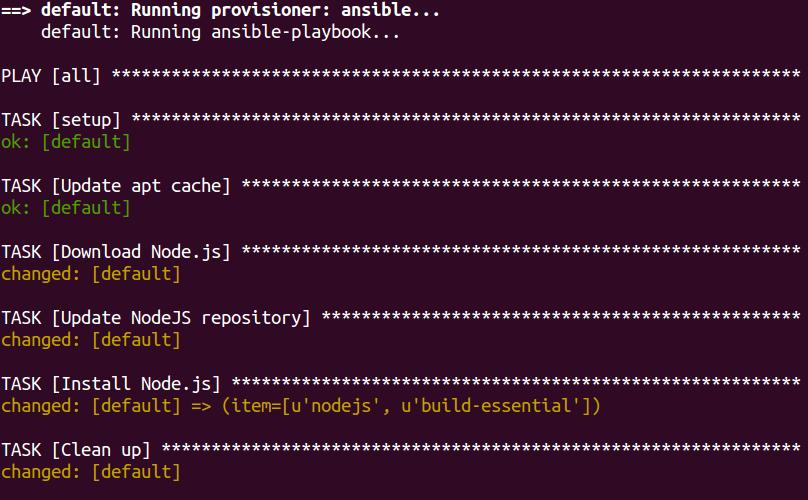
\includegraphics[width=\textwidth]{ansible-running}
  \caption{Ansible tuloste kun se ajaa tehtäviä}
  \label{fig:ansible-running}
\end{figure}

\begin{figure}[h]
  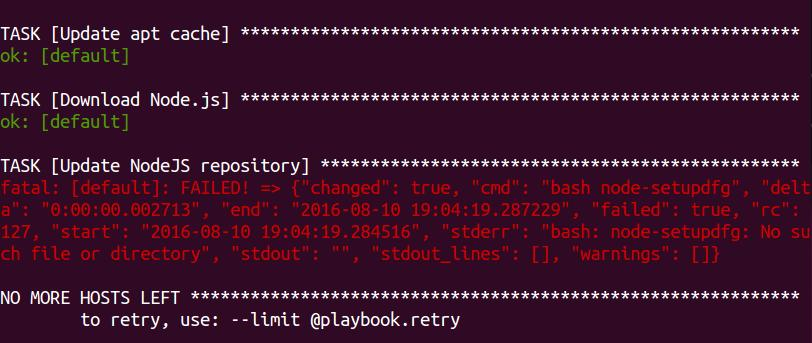
\includegraphics[width=\textwidth]{ansible-fails}
  \caption{Ansiblen tehtävä epäonnistuu}
  \label{fig:ansible-fails}
\end{figure}

\begin{figure}[h]
  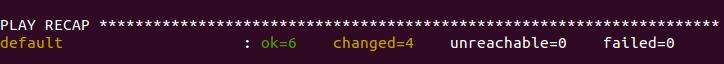
\includegraphics[width=\textwidth]{ansible-summary}
  \caption{Ansiblen yhteenveto tehtävien suorituksesta}
  \label{fig:ansible-summary}
\end{figure}

\begin{lstlisting}[
  label=listing:final-node-vagrantfile,
  language=Ruby,
  caption=Lopullinen Vagrantfile Node virtuaalikoneelle,
  float=h
]
Vagrant.configure(2) do |config|
  config.vm.box = "ubuntu/trusty64"

  config.vm.network "forwarded_port", guest: 8080, host: 3000

  config.vm.synced_folder ".", "/vagrant"

  config.vm.provision "ansible" do |ansible|
    ansible.playbook = "playbook.yml"
  end
end
\end{lstlisting}

\begin{lstlisting}[
  label=listing:node-server,
  language=JavaScript,
  caption=Yksinkertainen Node-palvelin,
  float=h
]
const http = require('http');

const PORT = 8080;

function handleRequest(request, response) {
  response.end(`It Works!! Path Hit: ${request.url}`);
}

const server = http.createServer(handleRequest);

server.listen(PORT, () => {
  console.log(`Server listening on: http://localhost:${PORT}`);
});
\end{lstlisting}

\begin{figure}[h]
  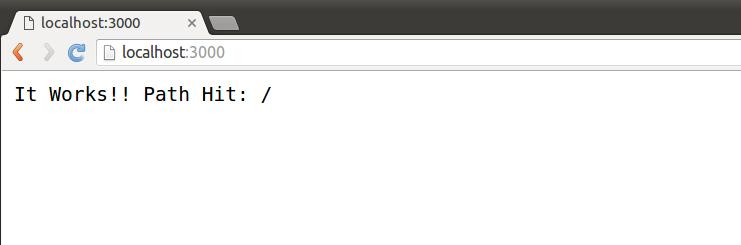
\includegraphics[width=\textwidth]{node-server-response}
  \caption{Node-palvelimen vastaus isäntäkoneessa}
  \label{fig:node-server-response}
\end{figure}

\subsection{Ansible oikeassa maailmassa}


Muista kertoa ansiblen sivusta galaxy.ansible.com
	
  \chapter{Yhteenveto}

Insinöörityön tarkoituksena oli ratkaista yleisimpiä kehitysympäristöön liittyviä ongelmia. Suurin osa näistä ongelmista johtuu paikalliseen koneeseen asennetuista käyttöjärjestelmäherkistä ohjelmista. Näin syntyy usein \enquote{toimii minun koneellani -tilanteita}. Insinöörityössä esitettiin ratkaisuja miten erilaisia kehitysympäristöjä virtualisoimalla päästään eroon yleisimmistä ongelmista.

Työssä käytettiin Vagrant-ohjelmaa luomaan yhtenäisiä virtuaalikoneita, joiden luomisprosessi voidaan kuvata koodina ja jotka voidaan versioida projektin versionhallintaan. Näin virtuaalikoneet ovat helposti jaettavia tiimin kesken. Ensiksi kerrottiin vertauskuvan ja kaavioiden avulla miten Vagrant toimii. Sen jälkeen käytiin yksityiskohtaisesti käytännön tasolla läpi miten voidaan luoda yksinkertainen virtuaalikone Apache- ja Node-ympäristöön. Insinöörityössä mainittiin myös Vagrantin huonot puolet kuten raskas muistin käyttö ja ongelmat isäntäkoneen ollessa Windows.

Insinöörityön jälkimmäisessä osassa tutustuttiin Ansibleen, joka helpottaa virtuaalikoneiden asennusta verrattuna shell-skripteihin. Ansiblen tapauksessakin ensi selitettiin Ansiblen hyöty vertauskuvana ja sen jälkeen sama asia selitettiin kaavioiden avulla. Selitysten jälkeen paranneltiin Vagrant osiossa luotuja virtuaalikoneita muuttamalla sen ohjelmien asennus Ansiblen mukaisiksi. Lopputuloksena oli  hyvin modulisoitu playbook, jonka osia voi helposti käyttää muissakin projekteissa, joissa tarvitaan samoja ohjelmia kuin testiprojektissa.

Kaiken kaikkiaan insinöörityö on antanut lukijalle valmiudet jatkaa virtuaaliympäristöjen tutkimista. Virtuaaliympäristöjen hyödyt kannattaa ottaa heti käyttöön, sillä nykyisillä työmarkkinoilla näiden taitojen hallitseminen on tärkeää.	
  
  \renewcommand{\bibname}{Lähteet}
\bibliographystyle{vancouver}
\bibliography{references}
\end{document}